%%% TeX-command-extra-options: "-shell-escape"
%!TEX options=--shell-escape

%----------------------------------------------------------------------------------------
%   PACKAGES AND THEMES
%----------------------------------------------------------------------------------------
\documentclass[aspectratio=169,xcolor=dvipsnames]{beamer}
% \usetheme{Simple}
\usepackage[english]{babel}
\usepackage{pgfpages}

%\setbeameroption{show notes}
\setbeameroption{show notes on second screen}
\setbeamertemplate{note page}[plain]

\usepackage{hyperref}
\usepackage{graphicx} % Allows including images
\usepackage{booktabs} % Allows the use of \toprule, \midrule and \bottomrule in tables

% hyperlinks
\usepackage{hyperref}
\hypersetup{
    colorlinks=true,
    linkcolor=, % no color for internal links
    filecolor=magenta,
    urlcolor=blue,
}

% code
% \usepackage{minted}
% \setminted{
%     fontsize=\footnotesize,
%     autogobble,
%     bgcolor=mygray,
%     fontsize=\small
% }

% colors
\usepackage{xcolor}
\definecolor{mygray}{gray}{0.95} % define color - grey scale: 0=dark - 1=light

% packages added with respect to overleaf
\usepackage[utf8]{inputenc}
\usepackage{lmodern}
\usepackage{textcomp}
\usepackage[most]{tcolorbox} % colored boxes

% custom commands
\definecolor{darkred}{HTML}{CC0000}
\newcommand\textveryimp[1]{\textcolor{darkred}{\underline{\textbf{#1}}}} % text bold+red+underlined
\newcommand\textimp[1]{\underline{\textbf{#1}}} % text bold+red+underlined
\newcommand\textcode[1]{\textcolor{gray}{\texttt{#1}}} % text typewriter font + gray

\newcommand\blfootnote[1]{%
  \begingroup
  \renewcommand\thefootnote{}\footnote{#1}%
  \addtocounter{footnote}{-1}%
  \endgroup
}

% figures
\usepackage{tikz}
% \usetikzlibrary{shapes,backgrounds}
\usepackage{animate}
%\usepackage{media9}
% equations
\usepackage{amsmath}
\usepackage{amssymb}
\usepackage{empheq}
\usepackage{makecell}

% images
\graphicspath{ {./images/} } % Relative path to image directory

% insert table of content before each section
% \AtBeginSection[]
% {
%     \begin{frame}
%         \frametitle{Table of Contents}
%         % \tableofcontents[currentsection]
%     \end{frame}
% }
% \setbeamertemplate{subsection in toc}[subsections numbered] % add numbers in front of subsections
% \setbeamertemplate{subsection in toc}{\leavevmode\leftskip=2em$\bullet$\hskip1em\inserttocsubsection\par} % add bullets in front of subsections
%\setbeamertemplate{subsection in toc}{\leavevmode\leftskip=3.2em\rlap{\hskip-2em\inserttocsectionnumber.\inserttocsubsectionnumber}\inserttocsubsection\par}
\setbeamertemplate{subsection in toc}{\leavevmode\leftskip=3.5em\rlap{\hskip-1.25em\inserttocsubsectionnumber.}\inserttocsubsection\par} % add indented subsection number

\setbeamerfont{frametitle}{size=\scriptsize} % Set slide title fontsize
\setbeamercovered{transparent} % Set text to be semi-transparent during sequential overlay


%----------------------------------------------------------------------------------------
%   TITLE PAGE
%----------------------------------------------------------------------------------------

\title[short title]{Introduction to Machine Learning}
\subtitle{Lecture 08}
\author{Automatic Image Analysis}
\titlegraphic{
  
\includegraphics[height=3cm]{cvlogo}
  
\includegraphics[height=3cm]{tublogo}
}
%\date{2021-04-23}


%----------------------------------------------------------------------------------------
%   PRESENTATION SLIDES
%----------------------------------------------------------------------------------------

\begin{document}

\begin{frame}
    \titlepage
\end{frame}


% ------------------------------------------------
\section{Introduction to Machine Learning}
%------------------------------------------------

\begin{frame}{Why do machine learning?}
  \begin{figure}
    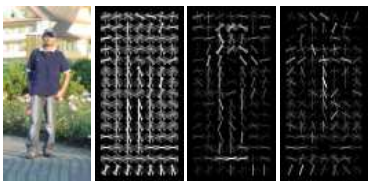
\includegraphics[width=0.8\textwidth]{hog}
  \end{figure}


  \note{
    \begin{itemize}
      \item How to connect our features to actual categories or measurements of image content in human terms?
      \item It would be hard to write heuristics to describe which HOG/SIFT feature corresponds to a dog or cat.
      \item There are two reason to make this connection.
            One is prediction of responses for unseen data.
            The other to analyze the connection between $x$ and $y$ (in statistics called inference).
      \item Image from Histograms of oriented gradients for human detection, Dalal \& Triggs
    \end{itemize}
  }
\end{frame}


\begin{frame}{What is machine learning?}

  \begin{figure}
    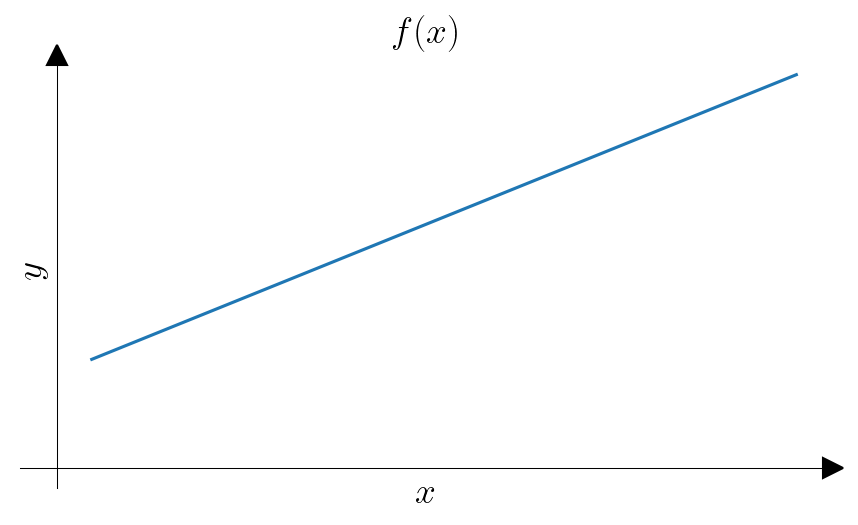
\includegraphics[width=0.8\textwidth]{ftrue}
  \end{figure}

  \note{
    \begin{itemize}
      \item We assume that there is a true mapping $f$ that maps from the image or feature space (predictor $x$) to e.g. an object category (response $y$).
      \item $x$ is also often called feature, input variable, just variable or independent variable.
      \item $y$ is also often called ground truth, target, label, output variable or dependent variable
      \item In the following we will often consider $x$ and $y$ to be multidimensional but visualize them mostly as scalars.
    \end{itemize}
  }
\end{frame}


\begin{frame}{What is machine learning?}

  \begin{figure}
    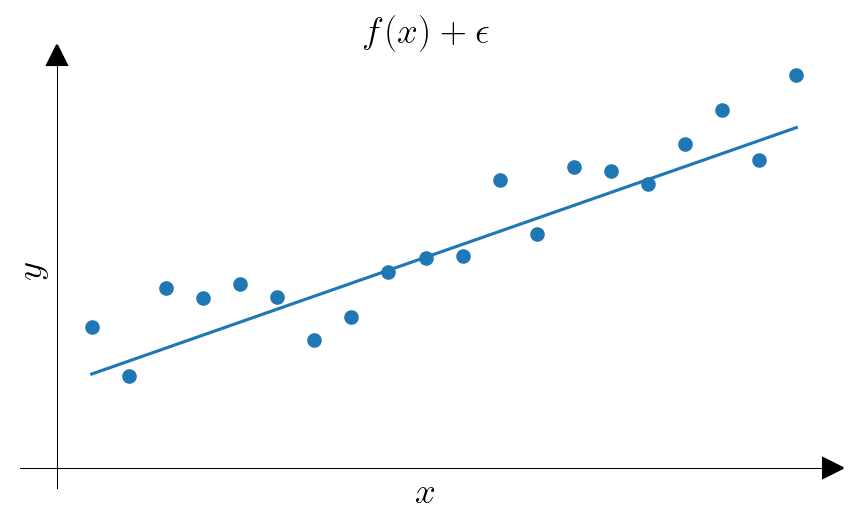
\includegraphics[width=0.8\textwidth]{feps}
  \end{figure}

\note{
  \begin{itemize}
    \item We want to estimate this function based on data we collected.
    \item When data is collected, we make an error $\epsilon$.
    \item This error is almost always of probabilistic nature. Our data is noisy.
    \item The set of measurements is denoted by $(Y, X)$ with all values collected for $X$ and their corresponding $y$s in $Y$.
  \end{itemize}
}
\end{frame}


\begin{frame}{Non-parametric Methods}

  \begin{figure}
    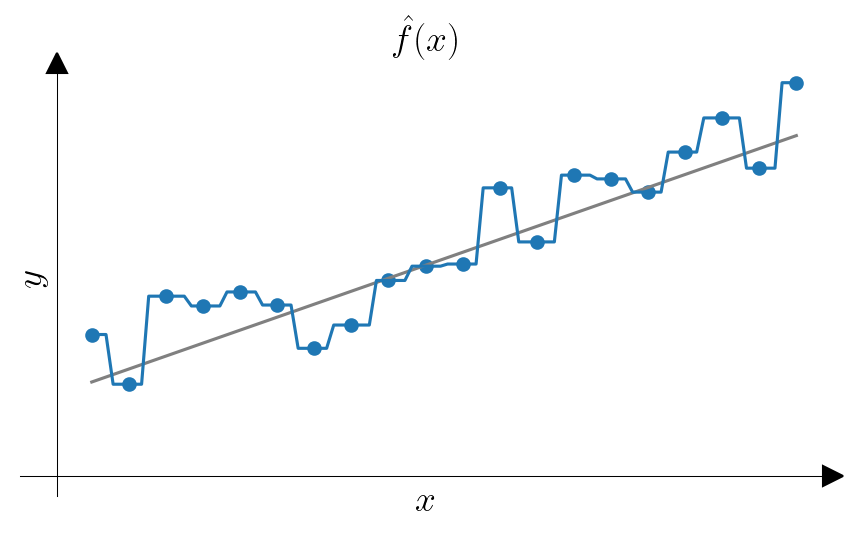
\includegraphics[width=0.8\textwidth]{fnoparam}
  \end{figure}
\note{
  \begin{itemize}
    \item Modeling of a wide range of functional forms possible.
    \item Usually very high number of observations necessary.
    \item In this case simply $\hat{f}(x) = Y_{argmin(|X-x|)}$
  \end{itemize}
}
\end{frame}


\begin{frame}{Parametric Methods}

  \begin{figure}
    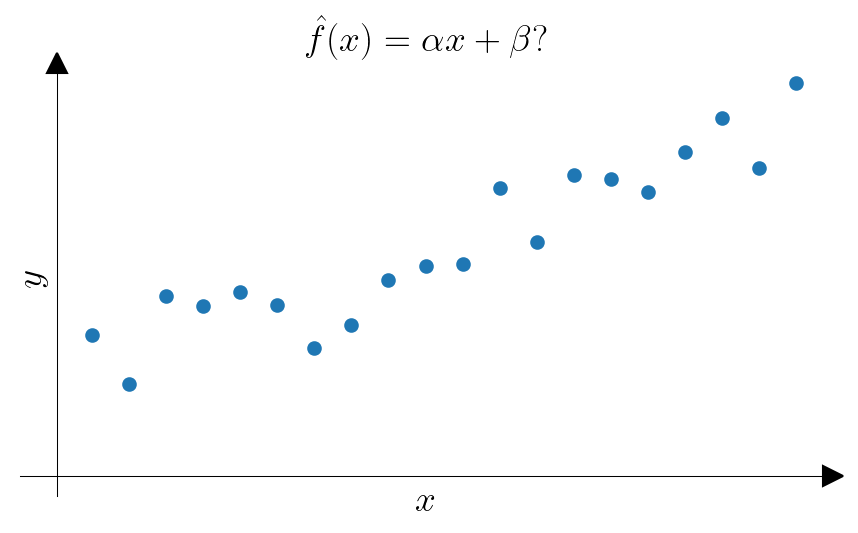
\includegraphics[width=0.8\textwidth]{fparam}
  \end{figure}
\note{
  \begin{itemize}
    \item We make an assumption about the functional form of $f$.
    \item In this case we might assume that the $f$ that generated our data is linear.
  \end{itemize}
}
\end{frame}


\begin{frame}{How can we estimate our parameters?}

  \vspace{1cm}
  \begin{equation*}
    E(\alpha, \beta) = \frac{1}{n}\sum_{i} (y_{i}-\hat{f}(x_{i}))^{2} = \frac{1}{n}\sum_{i} (y_{i}-\alpha x_{i} + \beta)^{2}
  \end{equation*}
\note{
  \begin{itemize}
    \item We need a criterion that tells us how well the estimation fits our data.
    \item An often used metric is the mean square error.
  \end{itemize}
}
\end{frame}

\begin{frame}{Linear Regression}

  \vspace{1cm}
  \begin{equation*}
    \frac{dE}{d\alpha} \stackrel{!}{=} 0 \text{ and } \frac{dE}{d\beta} \stackrel{!}{=} 0
  \end{equation*}
  \begin{align*}
    \hat{\alpha} & = \frac{\sum_{i}(x_{i}-\bar{x})(y_{i}-\bar{y})}{\sum_{i}(x_{i}-\bar{x})^{2}} \\
    \hat{\beta} & = \bar{y}-\hat{\alpha}\bar{x}
  \end{align*}
\note{
  \begin{itemize}
    \item To minimize the error, the first derivatives have to be zero.
    \item Using a linear model and mean square error allows for an analytical solution.
    \item Procedure is known as linear regression, a very simple and very popular method.
  \end{itemize}
}
\end{frame}


\begin{frame}
  \begin{figure}
    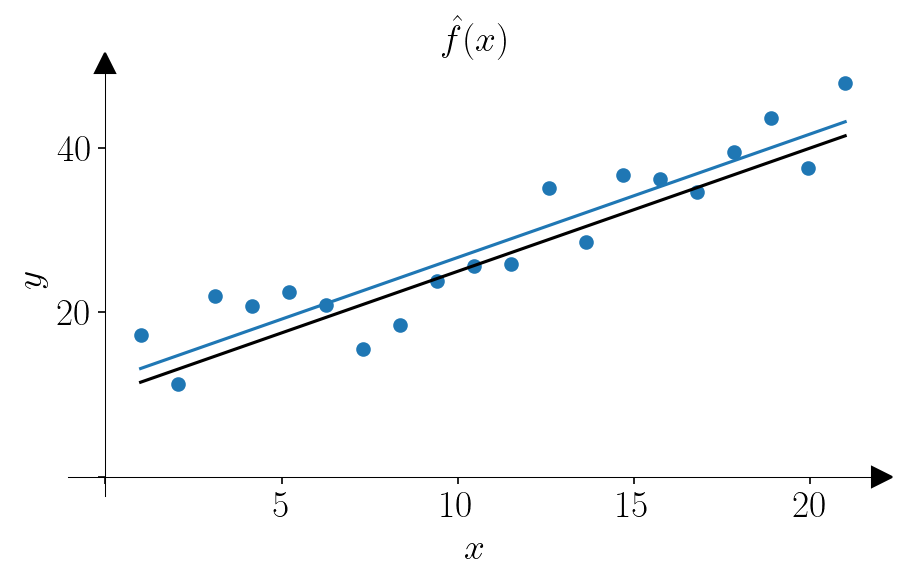
\includegraphics[width=0.8\textwidth]{linreg}
  \end{figure}
\note{
  \begin{itemize}
    \item Black shows the data generating ground truth, blue the estimate based on the measured data.
  \end{itemize}
}
\end{frame}


\begin{frame}{Error surface}

  \begin{figure}
    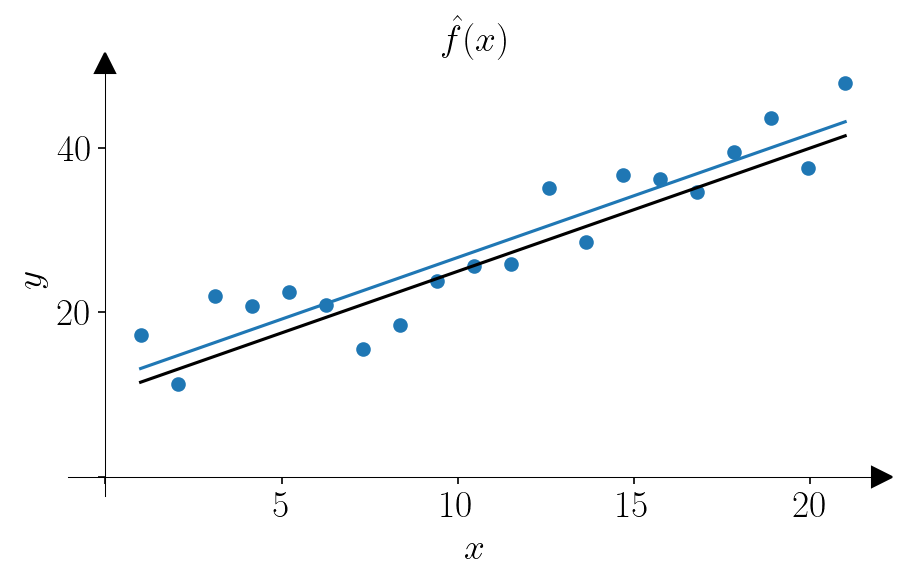
\includegraphics[width=0.4\textwidth]{linreg}
  \end{figure}
  \begin{figure}
    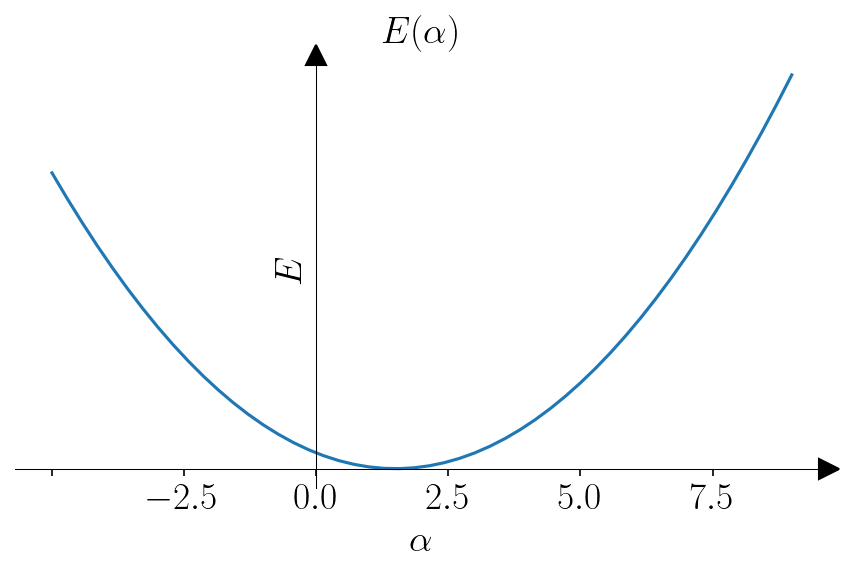
\includegraphics[width=0.4\textwidth]{erralpha}
    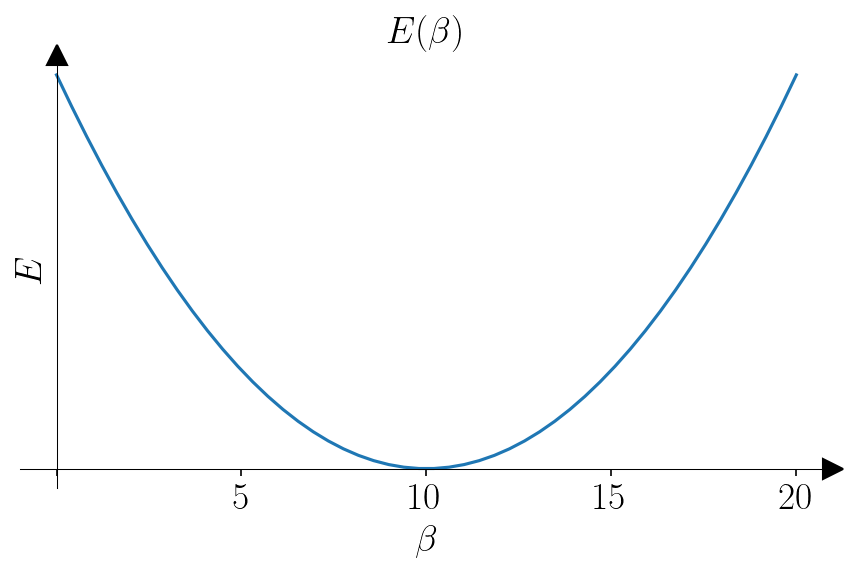
\includegraphics[width=0.4\textwidth]{errbeta}
  \end{figure}

\note{
  \begin{itemize}
    \item This slide shows the error surface of the linear model we just fitted to the data.
    \item On the left for the parameter alpha on the right for beta.
    \item We were lucky, not only has our problem a analytical solution it also has a convex error surface.
  \end{itemize}
}
\end{frame}


\begin{frame}{Error surface}

  \begin{figure}
    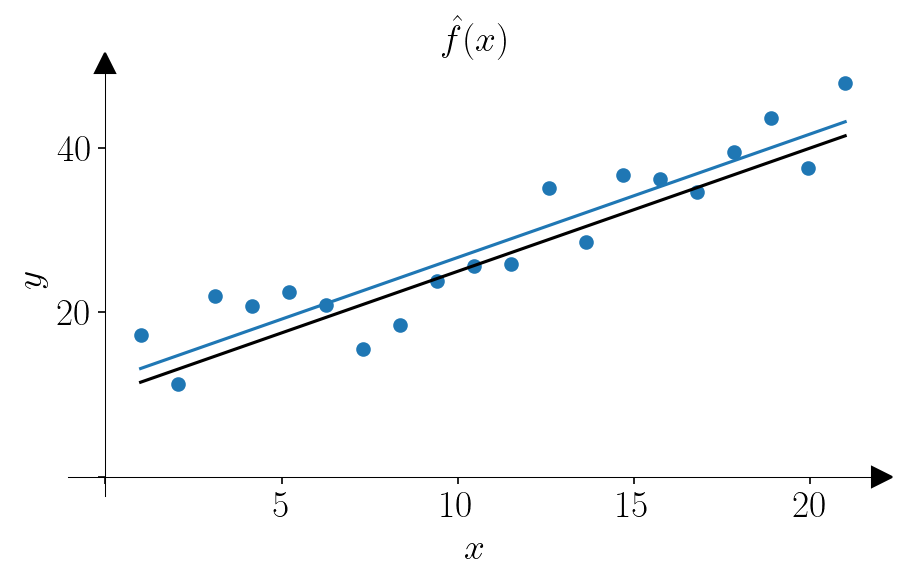
\includegraphics[width=0.4\textwidth]{linreg}
    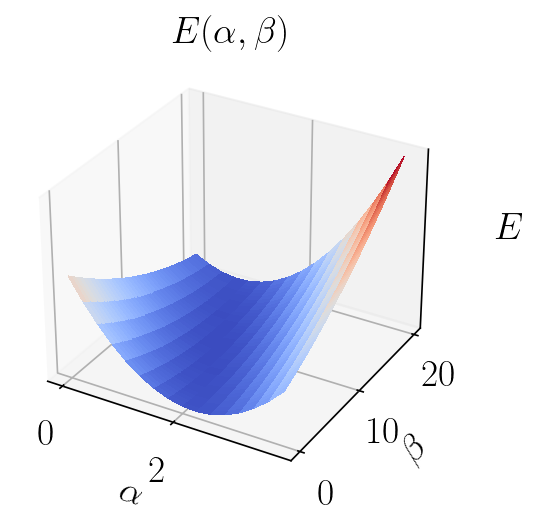
\includegraphics[width=0.4\textwidth]{err2d}
  \end{figure}

\note{
  \begin{itemize}
    \item Same function plotted in 2d.
    \item We were lucky, not only has our problem a analytical solution it also has a convex error surface.
  \end{itemize}
}
\end{frame}


\begin{frame}{Error surface}

  \begin{figure}
    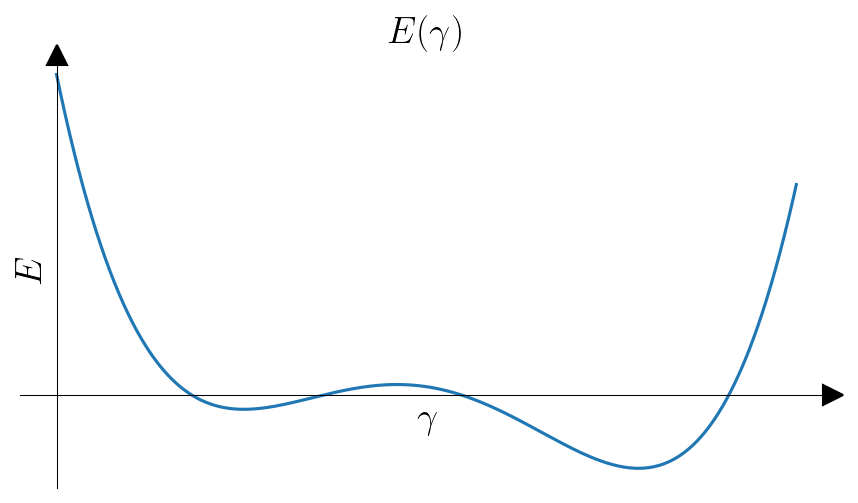
\includegraphics[width=0.8\textwidth]{nonconvex}
  \end{figure}

\note{
  \begin{itemize}
    \item Unfortunately, for more complex problems, this error surfaces are often non-convex.
    \item Especially when we can not find analytical solutions, local minima in such non-convex objective function can be problematic.
  \end{itemize}
}
\end{frame}


\begin{frame}{What if linear is not good enough?}

  \begin{figure}
    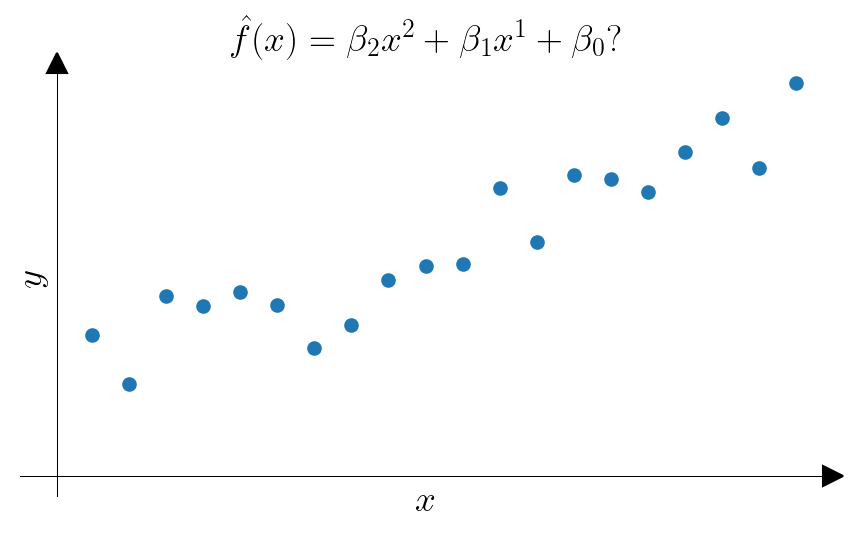
\includegraphics[width=0.8\textwidth]{fnonlin}
  \end{figure}
\note{
  \begin{itemize}
    \item A common pattern in machine learning is to apply linear methods trained on non-linear functions of the data.
    \item We map in a non-linear way to a higher dimensional features space and do linear regression.

  \end{itemize}
}
\end{frame}


\begin{frame}{What if linear is not good enough?}

  \begin{figure}
    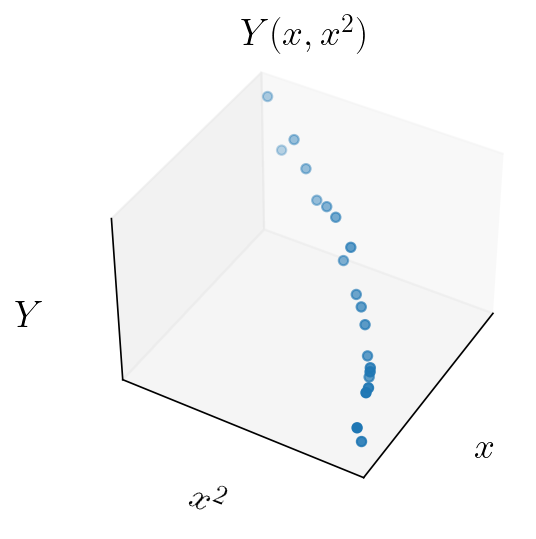
\includegraphics[width=0.3\textwidth]{fnonlin2da}
    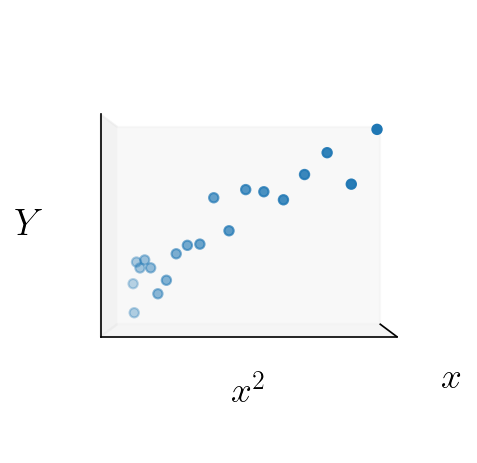
\includegraphics[width=0.3\textwidth]{fnonlin2db}
    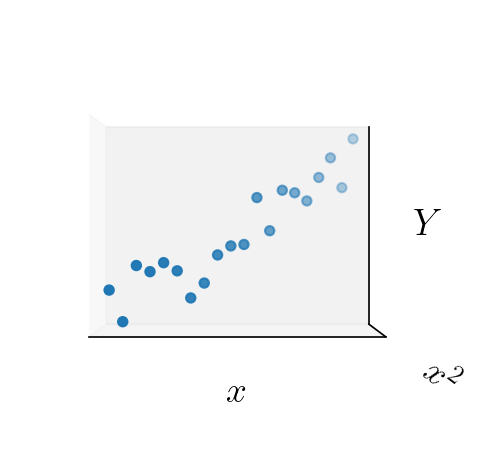
\includegraphics[width=0.3\textwidth]{fnonlin2dc}
  \end{figure}
\note{
  \begin{itemize}
    \item In our case we can map from our scalar feature space to $x' = (x, x^{2})$
    \item We see that relation between $x$ and $y$ stays the same while the $x^{2}$ dimension shows square root characteristics.
  \end{itemize}
}
\end{frame}


\begin{frame}{What if linear is not good enough?}

  \begin{figure}
    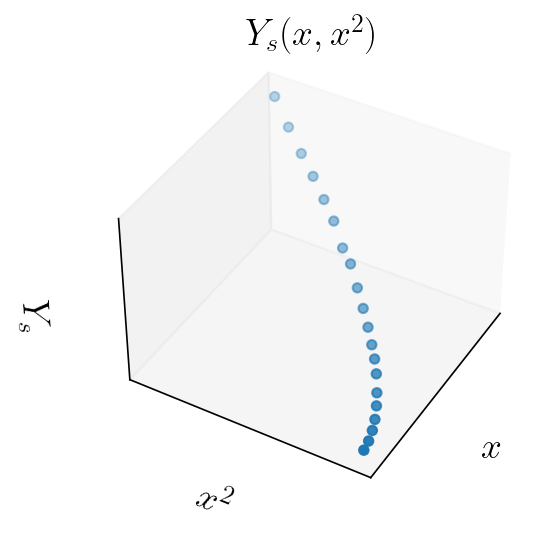
\includegraphics[width=0.3\textwidth]{fsquarenonlin2da}
    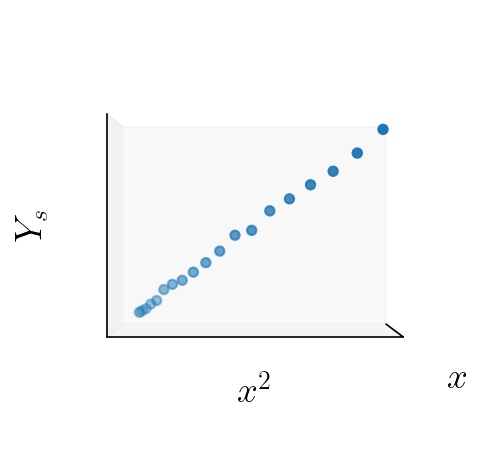
\includegraphics[width=0.3\textwidth]{fsquarenonlin2db}
    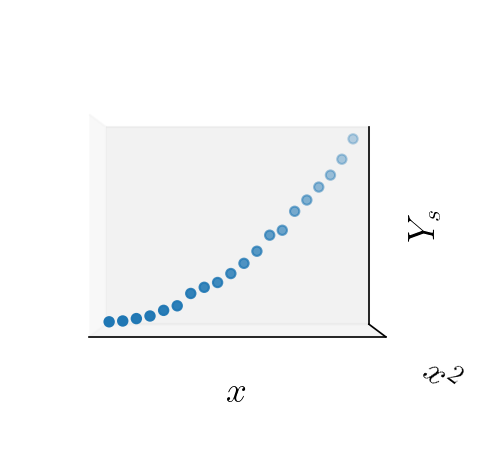
\includegraphics[width=0.3\textwidth]{fsquarenonlin2dc}
  \end{figure}
\note{
  \begin{itemize}
    \item On this slide the underlying $f$ from which the data is generated is $f(x)=x^{2}$.
    \item We see that relation between $x$ and $y$ is polynomial, while the $x^{2}$ dimension now is linear.
  \end{itemize}
}
\end{frame}


\begin{frame}{What if linear is not good enough?}

  \begin{figure}
    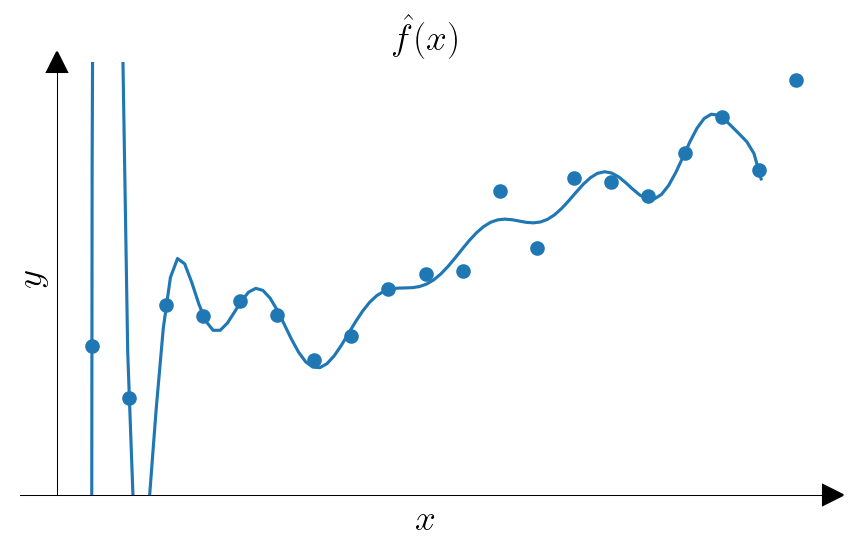
\includegraphics[scale=0.9]{fnonlinfit13}
  \end{figure}

\note{
  \begin{itemize}
    \item This slide shows a 17th degree polynomial fitted to our data from before.
    \item $y=f(x)+\epsilon=\frac{3}{2}x+10+\mathcal{N}(0, 4)$
  \end{itemize}
}
\end{frame}



\begin{frame}{Overfitting}

  \begin{figure}
    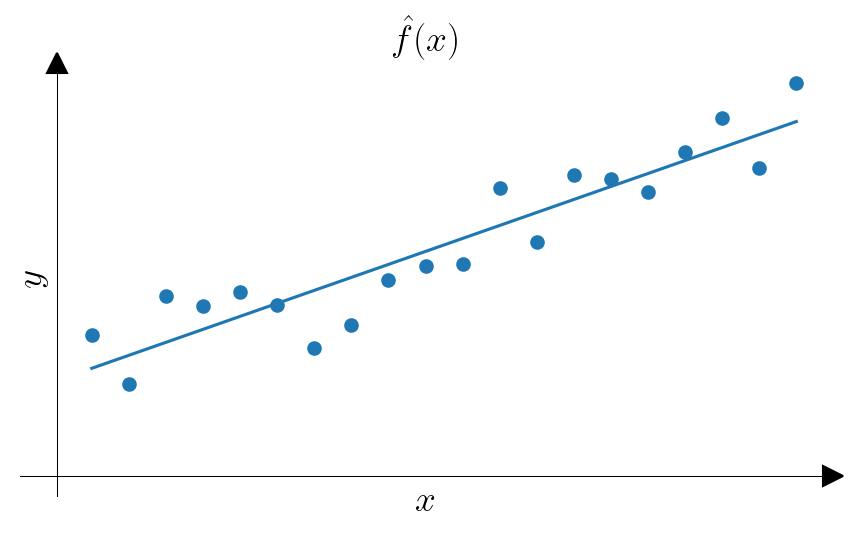
\includegraphics[width=0.4\textwidth]{linregnoticks}
    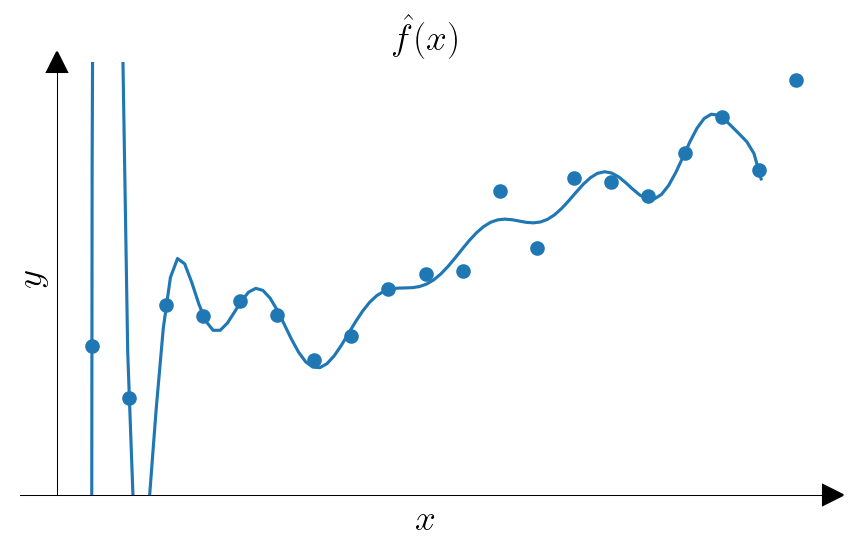
\includegraphics[width=0.4\textwidth]{fnonlinfit13}
  \end{figure}

\note{
  \begin{itemize}
    \item Which of the two estimates of $f$ is better?
    \item $y=f(x)+\epsilon=\frac{3}{2}x+10+\mathcal{N}(0, 4)$
  \end{itemize}
}
\end{frame}


\begin{frame}{Underfitting}

  \begin{figure}
    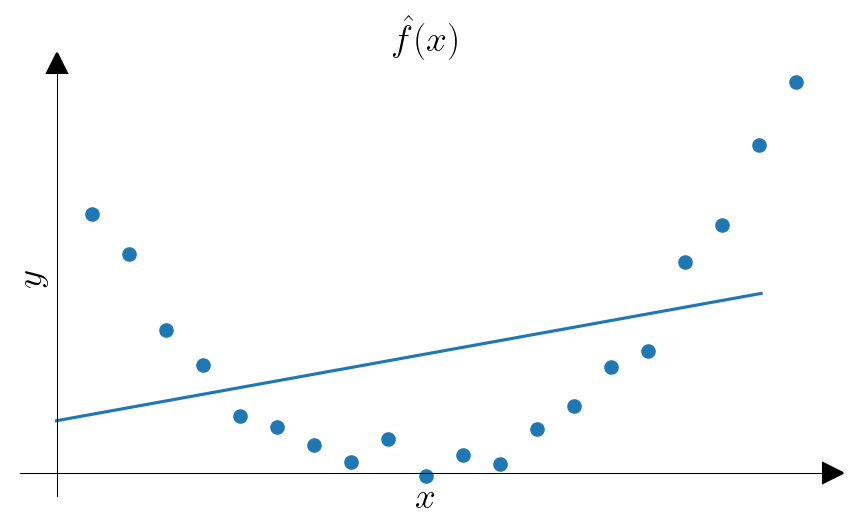
\includegraphics[width=0.4\textwidth]{flnsq}
    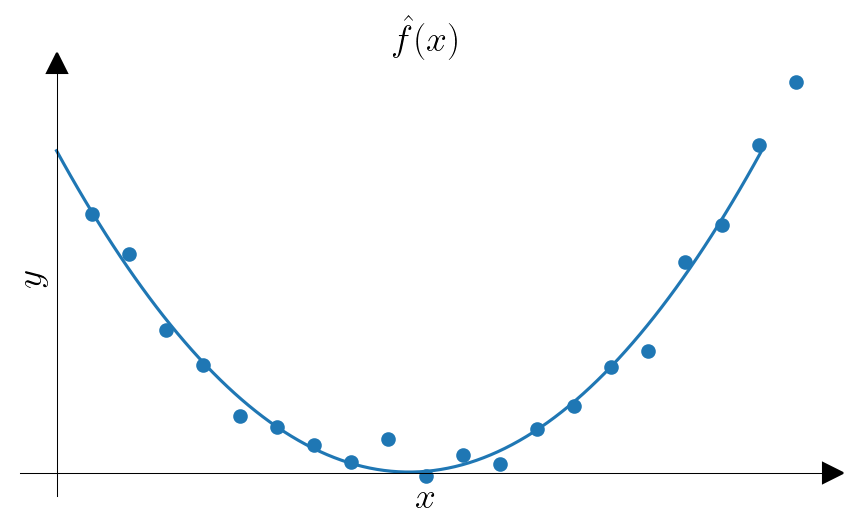
\includegraphics[width=0.4\textwidth]{fsqsq}
  \end{figure}

\note{
  \begin{itemize}
    \item Which of the two estimates of $f$ is better?
    \item $y=f(x)+\epsilon=4(x-10)^{2}+\mathcal{N}(0, 4)$
  \end{itemize}
}
\end{frame}


\begin{frame}{Bias-Variance Trade-Off: Bias}

  \begin{figure}
    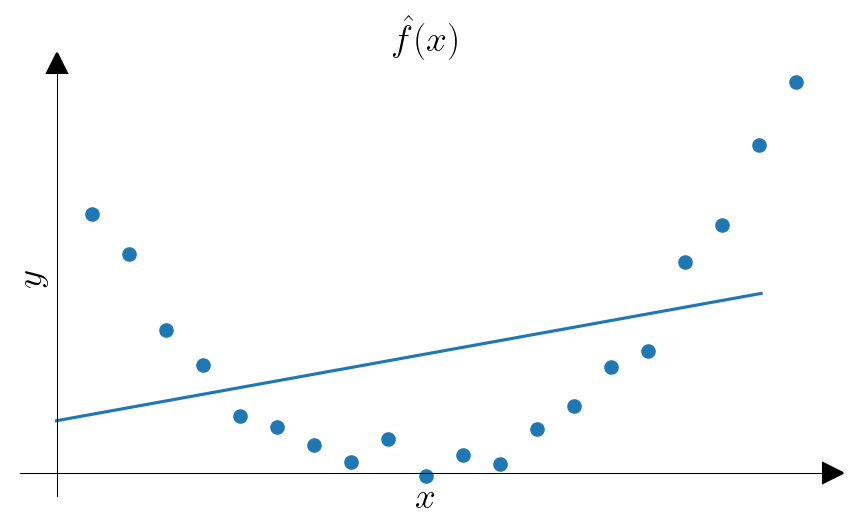
\includegraphics[width=0.4\textwidth]{flnsq}
    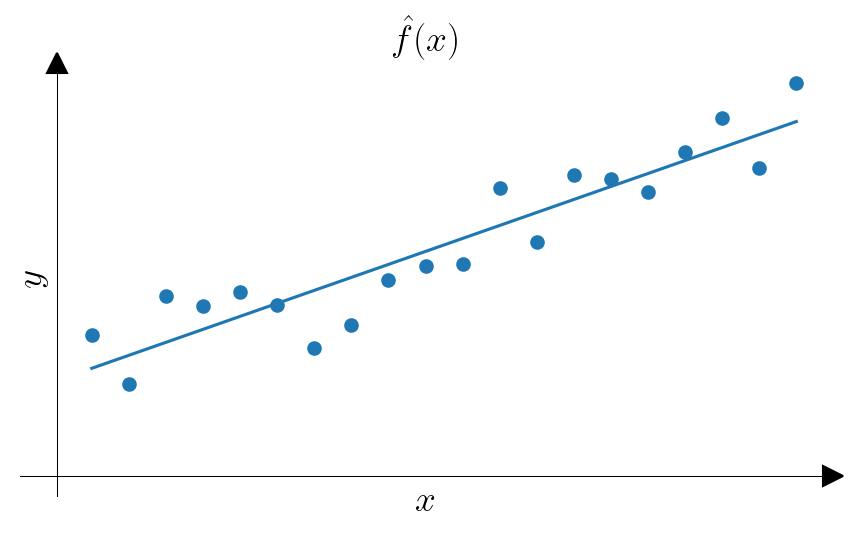
\includegraphics[width=0.4\textwidth]{linregnoticks}
  \end{figure}

\note{
  \begin{itemize}
    \item If we restrict our model e.g. by limiting the complexity we call that bias.
    \item In this case the model is limited to learn linear mappings (high bias).
  \end{itemize}
}
\end{frame}


\begin{frame}{Bias-Variance Trade-Off: Variance}

  \begin{figure}nnnn
    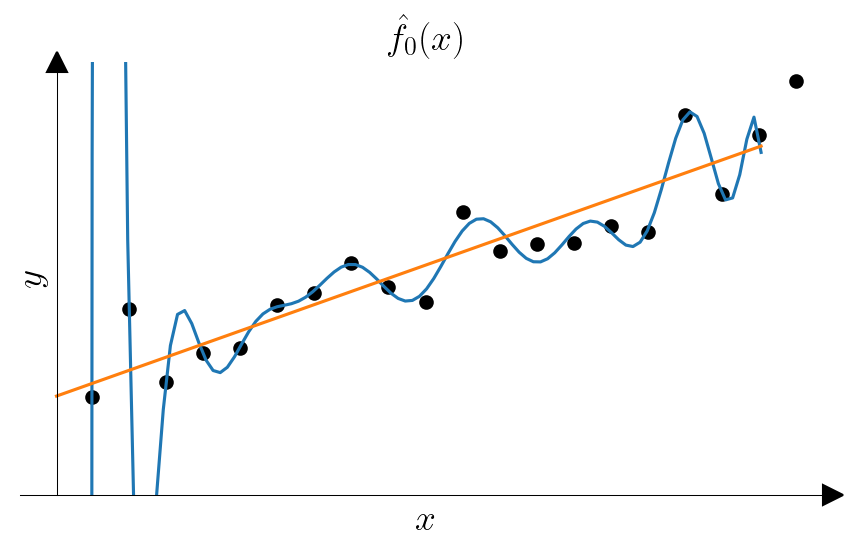
\includegraphics[width=0.3\textwidth]{variance0}
    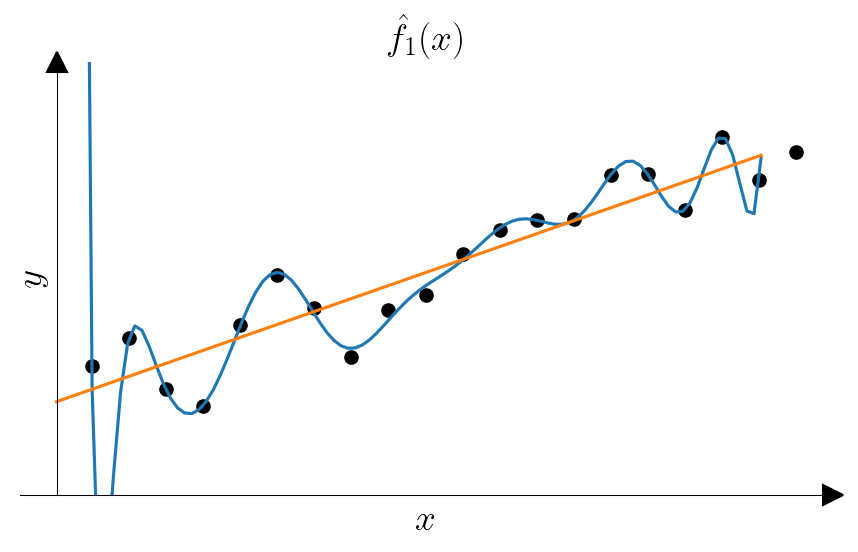
\includegraphics[width=0.3\textwidth]{variance1}
    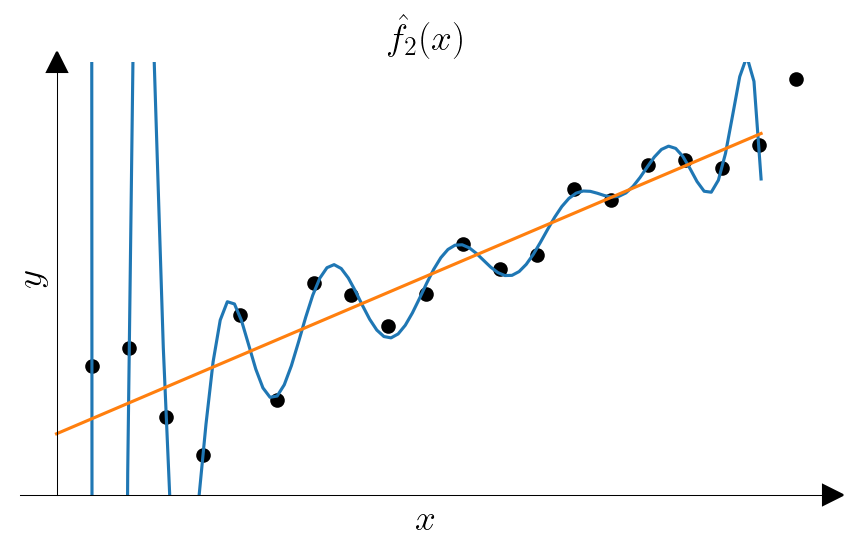
\includegraphics[width=0.3\textwidth]{variance2}
  \end{figure}

\note{
  \begin{itemize}
    \item Three different datasets. Each generated with the linear $f$ we used above.
    \item A 17th degree polynomial is fitted to each of them.
    \item We observe a high variance in the resulting polynomials.
    \item $y=f(x)+\epsilon=\frac{3}{2}x+10+\mathcal{N}(0, 4)$
  \end{itemize}
}
\end{frame}


\begin{frame}{Bias-Variance Trade-Off: Variance}

  \begin{figure}
    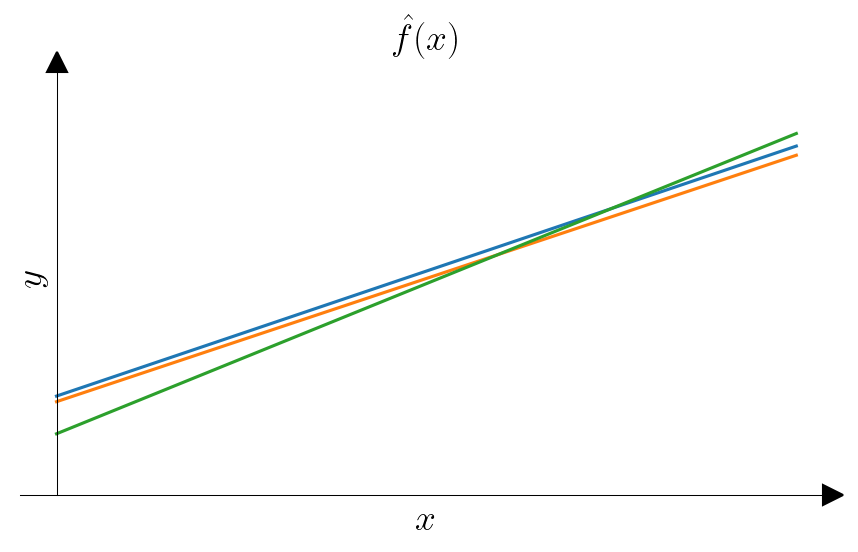
\includegraphics[width=0.4\textwidth]{varianceallln}
    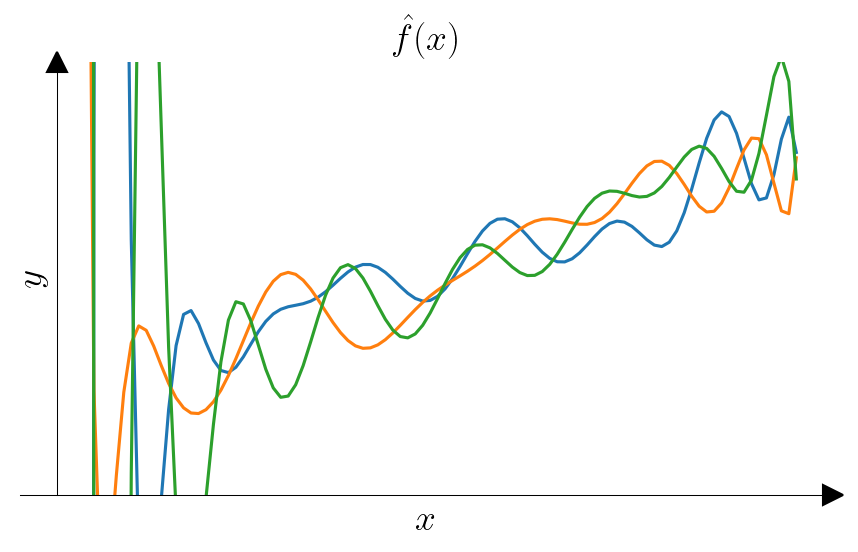
\includegraphics[width=0.4\textwidth]{varianceallsq}
  \end{figure}

\note{
  \begin{itemize}
    \item Three different datasets. Each generated with the linear $f$ we used above.
    \item Comparison on linear models versus polynomial models fitted to the same data.
  \end{itemize}
}
\end{frame}


\begin{frame}{Bias-Variance Trade-Off}

  \begin{figure}
    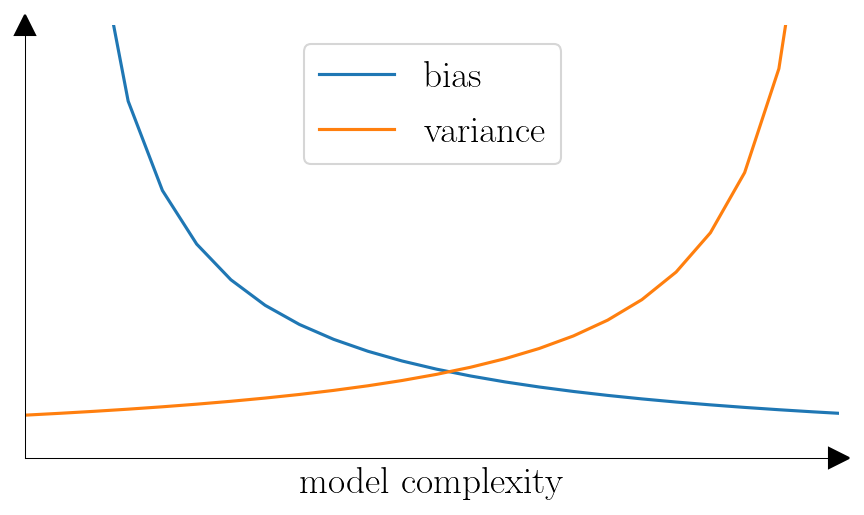
\includegraphics[width=0.9\textwidth]{biasvariance}
  \end{figure}

\note{
  \begin{itemize}
    \item Higher model complexity leads to higher variance and lower bias.
  \end{itemize}
}
\end{frame}


\begin{frame}{Model quality}

  \begin{figure}
    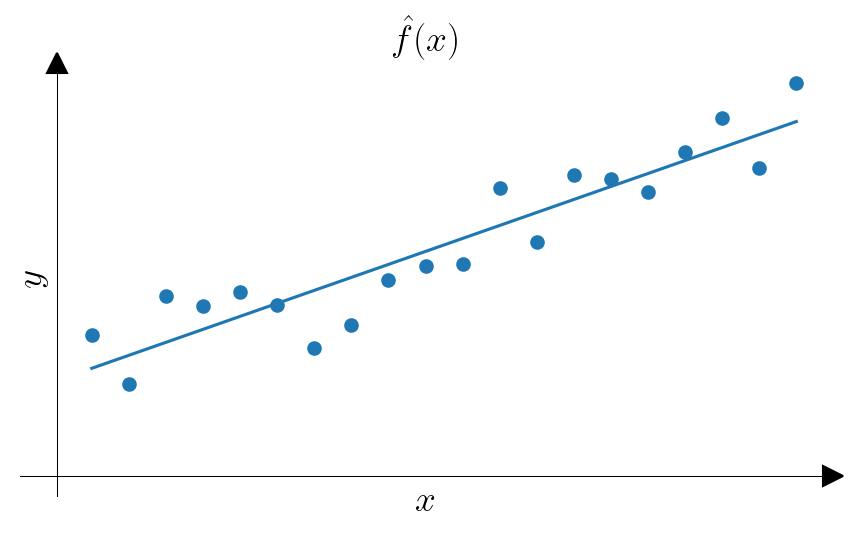
\includegraphics[width=0.4\textwidth]{linregnoticks}
    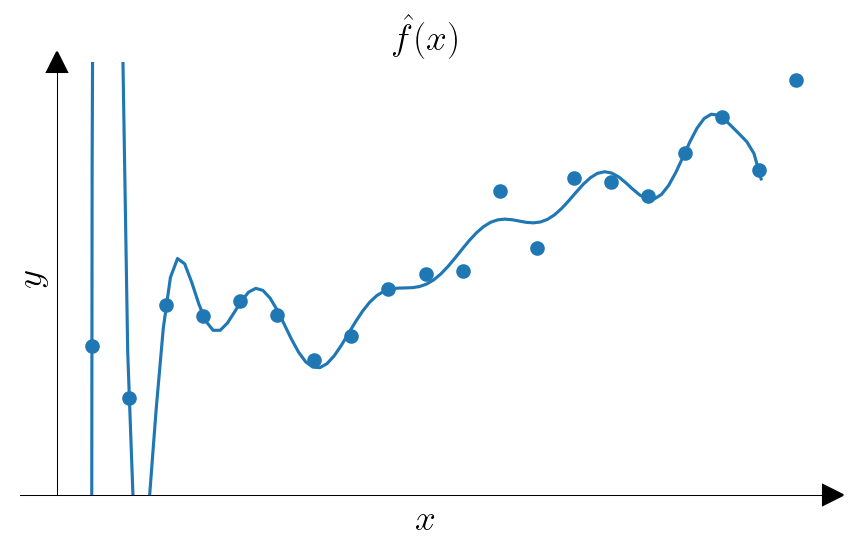
\includegraphics[width=0.4\textwidth]{fnonlinfit13}
  \end{figure}

\note{
  \begin{itemize}
    \item How can we measure the quality of our model?
    \item Which of the two is the better fit?
  \end{itemize}
}
\end{frame}


\begin{frame}{Model quality}
  \begin{equation}
    E = \frac{1}{n}\sum_{i} (y_{i}-\hat{f}(x_{i}))^{2}
  \end{equation}
  \begin{figure}
    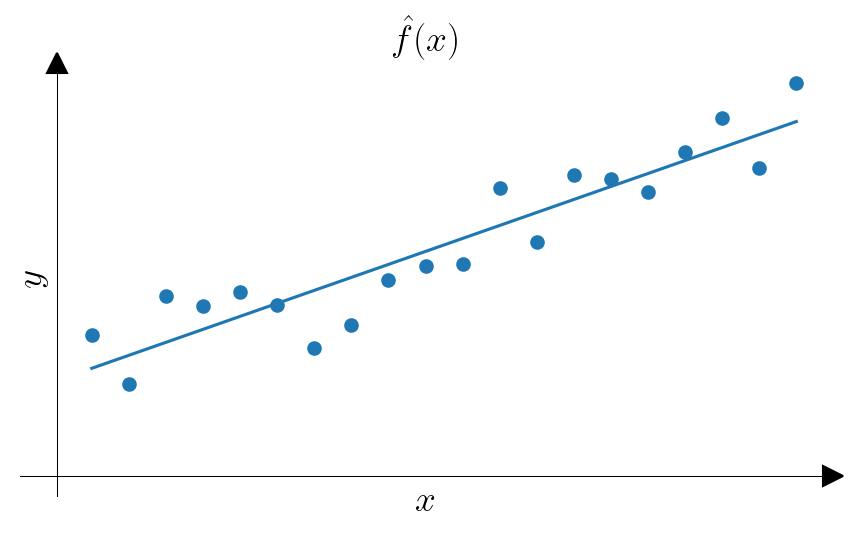
\includegraphics[width=0.4\textwidth]{linregnoticks}
    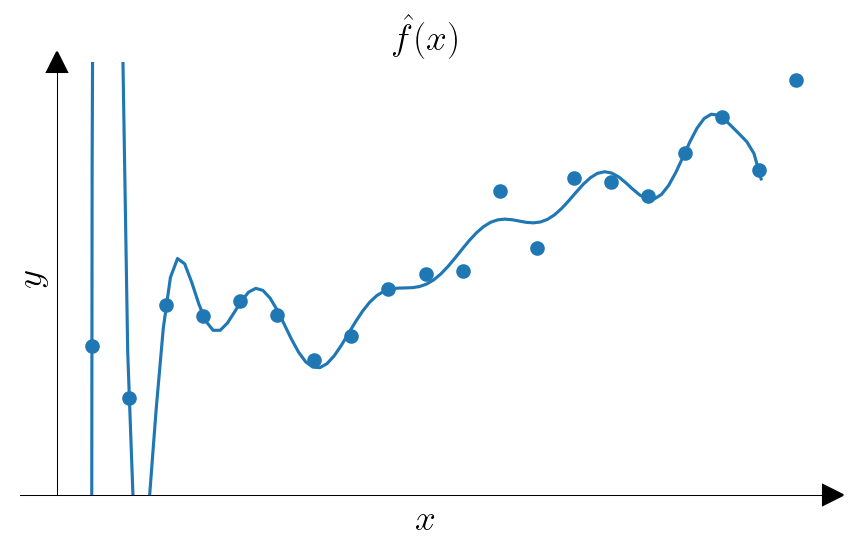
\includegraphics[width=0.4\textwidth]{fnonlinfit13}
  \end{figure}

\note{
  \begin{itemize}
    \item Which of the two has the smaller error (does minimize our objective)? \\
    $rightarrow$ Error becomes smaller with increasing model complexity.
  \end{itemize}
}
\end{frame}


\begin{frame}{Model quality: test dataset}

  \begin{equation}
    E = \frac{1}{n}\sum_{i} (y_{i}-\hat{f}(x_{i}))^{2}
  \end{equation}
  \begin{figure}
    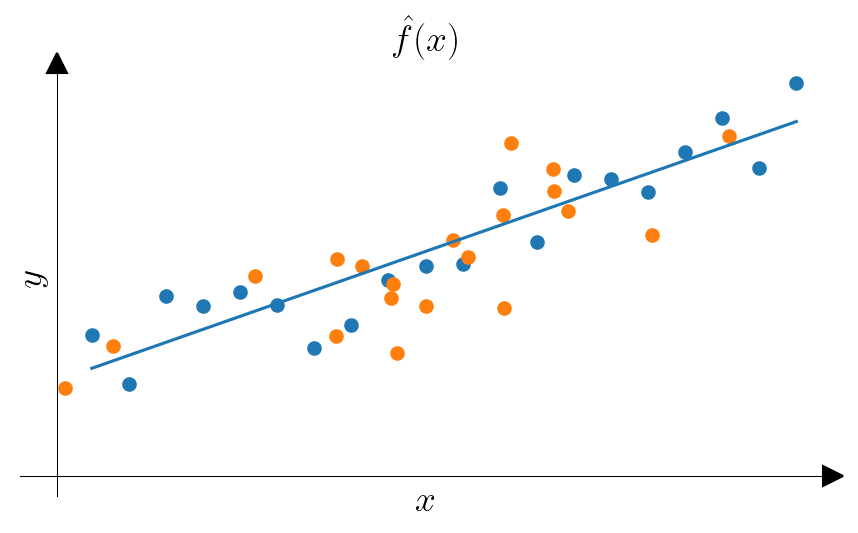
\includegraphics[width=0.4\textwidth]{linval}
    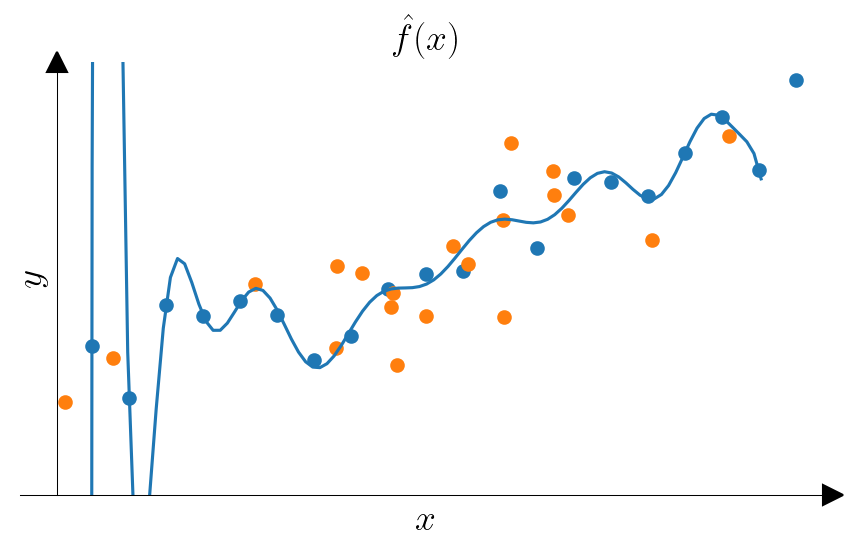
\includegraphics[width=0.4\textwidth]{nonlinval}
  \end{figure}

\note{
  \begin{itemize}
    \item Which of the two has the smaller error (does minimize our objective)?
    \item Split data set before fitting the model and test on unseen data.
    $\rightarrow$  Error shows when model overfits the training data.
  \end{itemize}
}
\end{frame}


\begin{frame}
  \begin{figure}
    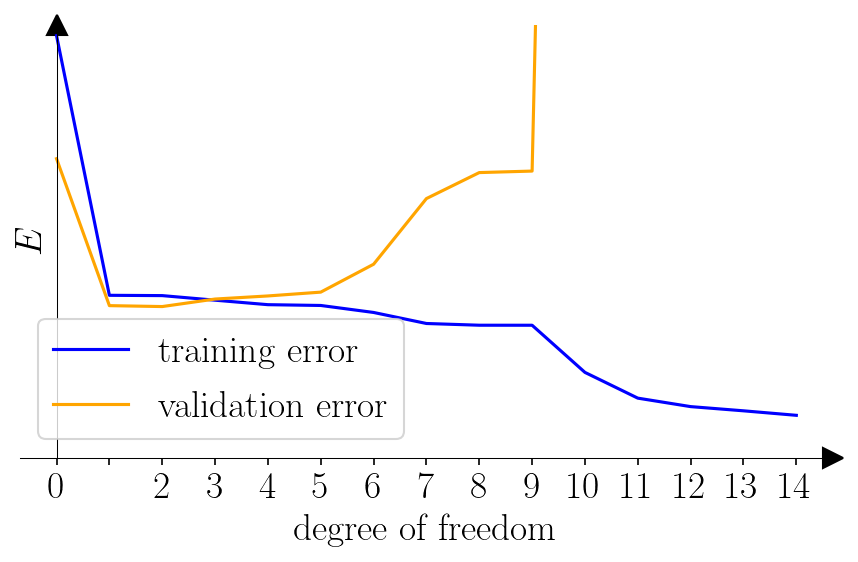
\includegraphics[width=0.9\textwidth]{trainvallin}
  \end{figure}

\note{
  \begin{itemize}
    \item A number of models with increasing complexity was fitted to some training data.
    \item What do you think what form the data generating distribution has?
  \end{itemize}
}
\end{frame}


\begin{frame}
  \begin{figure}
    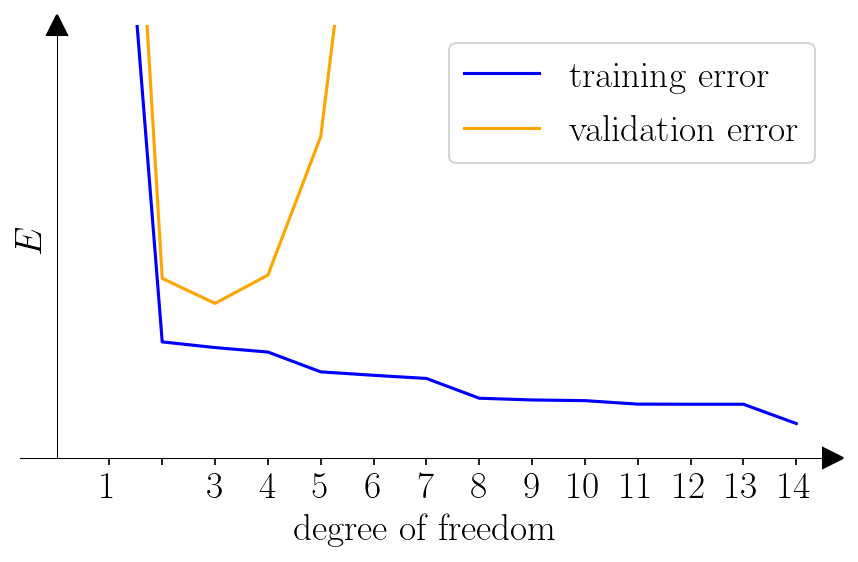
\includegraphics[width=0.9\textwidth]{trainvalpol}
  \end{figure}

\note{
  \begin{itemize}
    \item A number of models with increasing complexity was fitted to some training data.
    \item What do you think what form the data generating distribution has?
  \end{itemize}
}
\end{frame}



\begin{frame}{Classification}

  \begin{figure}
    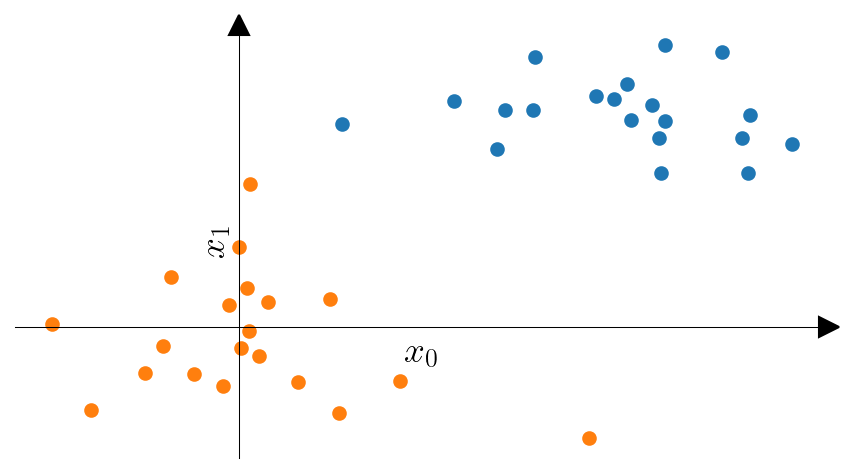
\includegraphics[width=0.9\textwidth]{classification}
  \end{figure}

\note{
  \begin{itemize}
    \item So far we looked at data were the response variable $y$ was quantitative. \\
    $\rightarrow$ This class of problems is referred to as regression problems.
    \item Now we want to look at problems were the response is qualitative or categorical.
    \item Examples: Categorization of facial expressions or objects in images.
  \end{itemize}
}
\end{frame}


\begin{frame}{Classification}
  \begin{figure}
    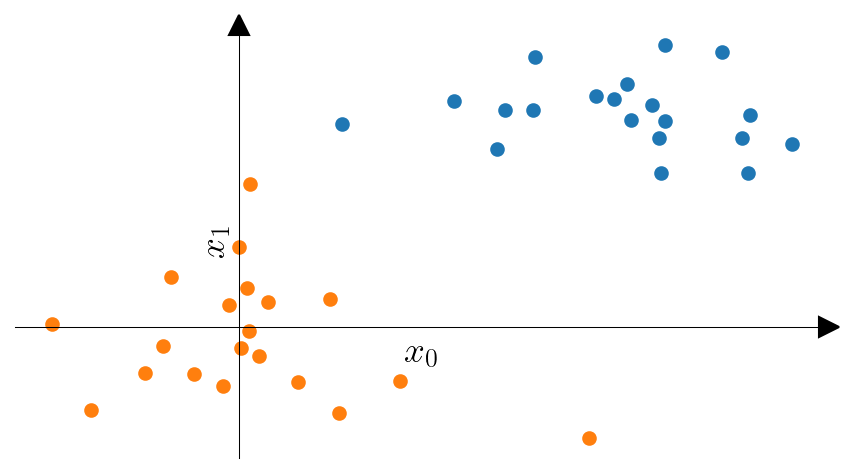
\includegraphics[width=0.9\textwidth]{classification}
  \end{figure}

\note{
  \begin{itemize}
    \item To do this our goal is it to identify a boundary in between a set of training points that separates the two classes.
    \item Whether we call a problem a classification or a regression problem depends only on the response variable.
    \item As for regression, we look only at quantitative predictor variables here.
    \item When the predictor variable is categorical as e.g. in natural language processing they are usually embedded in a quantitative space.
  \end{itemize}
}
\end{frame}


\begin{frame}{Can we solve this with Linear Regression?}

  \begin{figure}
    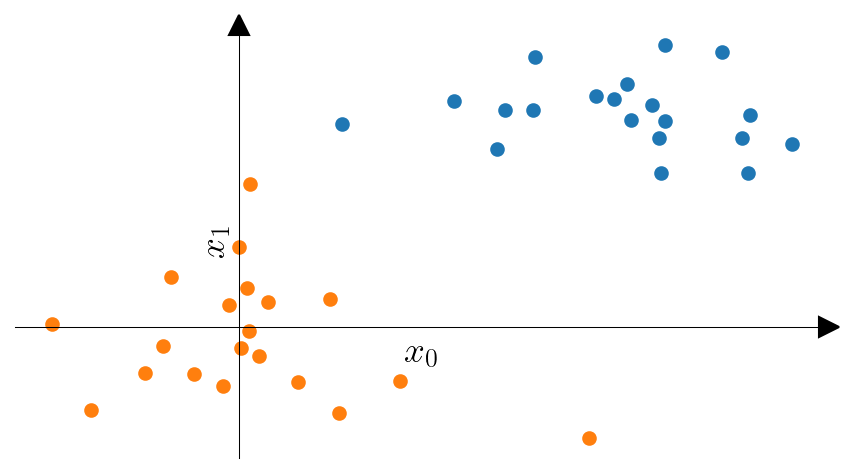
\includegraphics[width=0.9\textwidth]{classification}
  \end{figure}

\note{
  \begin{itemize}
    \item We could define the blue class label as $0$ and the orange class label as $1$ and then apply linear regression.
  \end{itemize}
}
\end{frame}


\begin{frame}{Can we solve this with Linear Regression?}

  \begin{figure}
    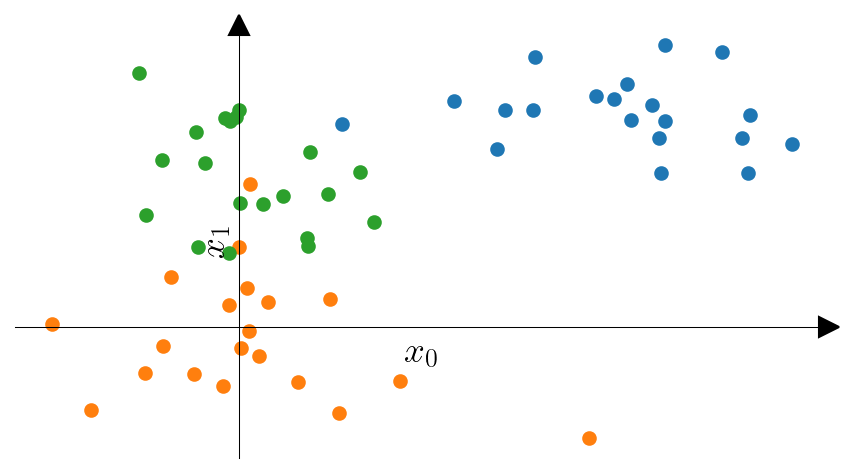
\includegraphics[width=0.9\textwidth]{classification_three}
  \end{figure}

\note{
  \begin{itemize}
    \item However, this would not generalize to more than the binary case.
    \item For three classes we cannot define and order as e.g. orange $>$ blue $>$ green, which would be implied if we would
          assign numbers to our classes as before.
  \end{itemize}
}
\end{frame}


\begin{frame}{Logistic Regression}

  \begin{equation}
    P(class=blue|x)
  \end{equation}
  \begin{figure}
    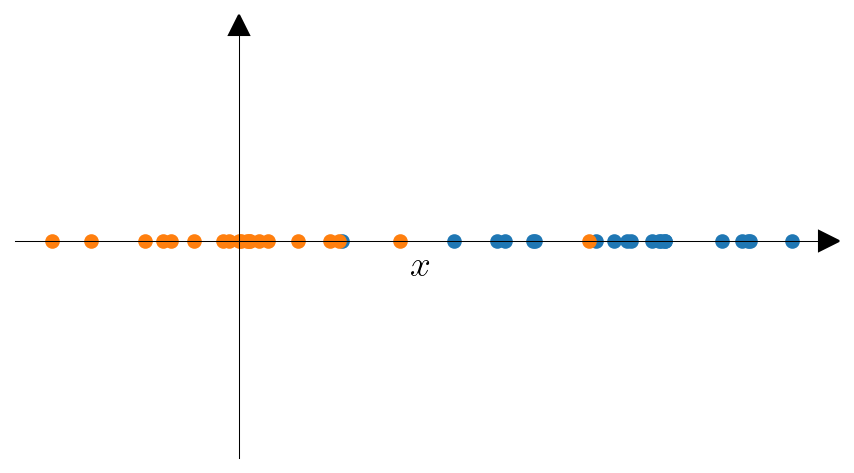
\includegraphics[width=0.9\textwidth]{classification_1d}
  \end{figure}

\note{
  \begin{itemize}
    \item There is a number of algorithms to approach this problem:
          LDA, SVM, Trees, Forests, K-nearest-neighbors, Boosting
    \item For this lecture however, we will first focus on Logistic Regression.
    \item The core idea is to formulate the problem as the regression of a probability function.
    \item This probability connects the predictor variables with the categorical response variable.
    \item For easier illustration, we switch to a two class problem with 1-dimensional input.
  \end{itemize}
}
\end{frame}


\begin{frame}{Logistic Regression}

  % \begin{equation}
  %   p(x) = \alpha x + \beta
  % \end{equation}
  \begin{figure}
    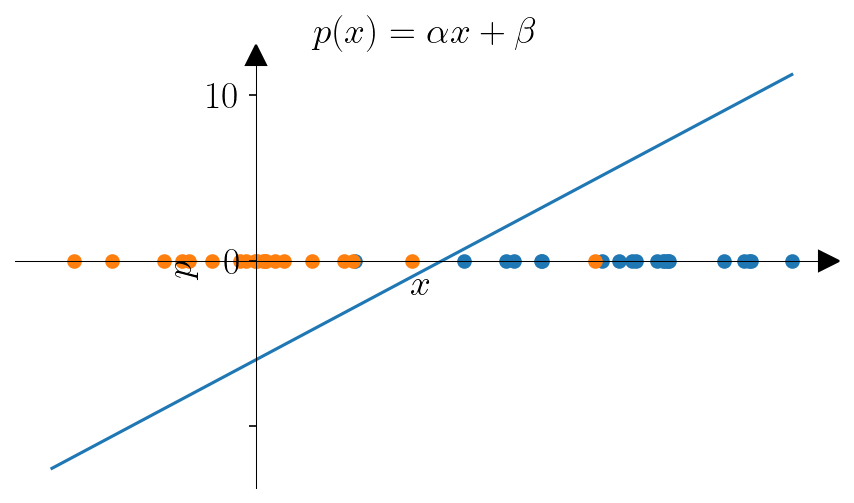
\includegraphics[width=0.8\textwidth]{classification_1d_linp}
  \end{figure}

\note{
  \begin{itemize}
    \item How to model the probability mass function? As a linear mapping as for the regression?
    \item $p$ gets arbitrarily big,  $> 1$ and $< 1$
  \end{itemize}
}
\end{frame}


\begin{frame}{Logistic Regression}

  % \begin{equation}
  %   p(c_{1}|x) = \frac{e^{\alpha x + \beta}}{1+e^{\alpha x + \beta}}
  % \end{equation}
  \begin{figure}
    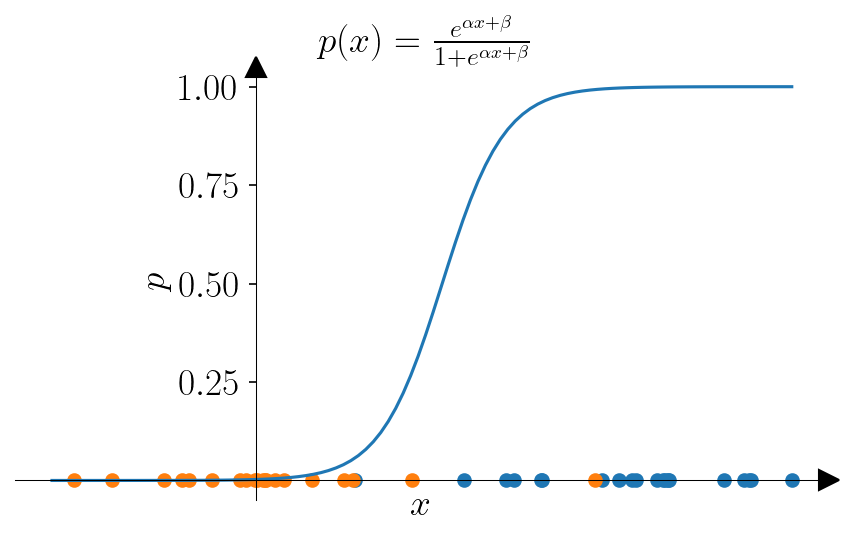
\includegraphics[width=0.8\textwidth]{classification_1d_logp}
  \end{figure}

\note{
  \begin{itemize}
    \item How to model the probability mass function? The logistic function is one of many that makes the result look more like a probability.
  \end{itemize}
}
\end{frame}


\begin{frame}{Logistic Regression}

  \begin{align*}
    p(blue|x) & =\frac{e^{\alpha x + \beta}}{1+e^{\alpha x + \beta}}\\
    p(orange|x) & =1-p(blue|x)
  \end{align*}
  \begin{figure}
    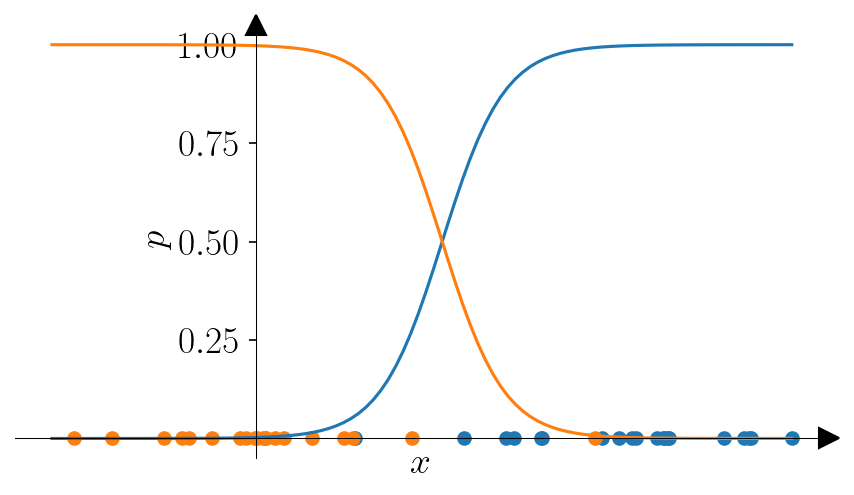
\includegraphics[width=0.7\textwidth]{classification_1d_logp_both}
  \end{figure}

\note{
  \begin{itemize}
    \item How to model the probability mass function? The logistic function is one of many that makes the result look more like a probability.
  \end{itemize}
}
\end{frame}


\begin{frame}{Logistic Regression: Maximum Likelihood}

  % \begin{align*}
  %   y = p(c_{1}|x) = \frac{e^{\alpha x + \beta}}{1+e^{\alpha x + \beta}}
  %   p(c_{0}|x) = 1 - p(c_{1}|x)  = 1 - \frac{e^{\alpha x + \beta}}{1+e^{\alpha x + \beta}}
  % \end{align*}

  \begin{align*}
    p(Y|X,\Theta) &= \prod_{\forall i} p(y_{i}|x_{i}) \\
    \log~p(Y|X,\Theta) &= \sum_{\forall i} \log~p(y_{i}|x_{i}) \\
    E(\Theta) = - \log~p(Y|X,\Theta) &= - \sum_{\forall i} \log~p(y_{i}|x_{i})
  \end{align*}

  % \begin{figure}
  %   \includegraphics[width=0.8\textwidth]{classification_1d_logp}
  % \end{figure}

\note{
  \begin{itemize}
    \item If the samples in our data set are independent and identically distributed (iid assumption) we can write the probability of our dataset beeing generated by our model as a product of the probabilities of the samples.
    \item In our case $\Theta =(\alpha, \beta)$.
    \item If we fix the data and vary the parameters $\Theta$, we call this the likelihood or log-likelihood respectively.
    \item We use the logarithm of the likelihood function for convenience.
    \item We define the error function as the negative log-likelihood and as for the linear regression we can use the derivatives of the error function to determine optimal estimates of $\alpha$ and $\beta$ for the given dataset.
  \end{itemize}
}
\end{frame}


\begin{frame}{Logistic Regression: cross entropy}

  \begin{align*}
    E(\Theta) &= - \sum_{\forall i} q(x) \log~p(y_{i}|x_{i}) = H(q, p)
  \end{align*}

\note{
  \begin{itemize}
    \item The resulting error function describes the cross entropy between the modeled probability distribution and the distribution $q$ which is $1$ if the sample belongs to the respective class and $0$ otherwise.
    \item For further reading we refer to Bishop p48ff.
  \end{itemize}
}
\end{frame}


\begin{frame}{Logistic Regression: softmax}

  \begin{align*}
    p_{i}(x) & = \sigma_{i}(x) = \frac{e^{z_{i}(x)}}{\sum_{\forall j}e^{z_{j}(x)}}
  \end{align*}
with
  \begin{align*}
    z_{i}(x) = \alpha_{i} x + \beta_{i}
  \end{align*}

\note{
  \begin{itemize}
    \item Using the $softmax$ function which is a generalization of the logistic function, we can apply logistic regression to multi class problems.
  \end{itemize}
}
\end{frame}


\begin{frame}{Logistic Regression: softmax}
  \begin{figure}
    \includegraphics[height=5cm]{classification_three_boundaries}
  \end{figure}

g  \begin{equation*}
    p(c|x, \Theta) =
    \begin{pmatrix}
      P(blue|x)\\
      P(orange|x)\\
      P(green|x)
    \end{pmatrix} = \sigma\left (
    \begin{pmatrix}
      \alpha_{00} & \alpha_{01} \\
      \alpha_{10} & \alpha_{11} \\
      \alpha_{20} & \alpha_{21}
    \end{pmatrix} \cdot
    \begin{pmatrix}
      x_0\\
      x_1\\
    \end{pmatrix} +
    \begin{pmatrix}
      \beta_0\\
      \beta_1\\
      \beta_2\\
    \end{pmatrix} \right )
  \end{equation*}

\note{
  \begin{itemize}
    \item Using the $softmax$ function which is a generalization of the logistic function, we can apply logistic regression to multi class problems.
    \item The matrix $\alpha_{ij}$ is often called the weight matrix $W$.
    \item The vector $\beta_{i}$ is often called the bias $b$.
    \item Such a classifier can be and often is written as $y=\sigma(Wx)$ w.l.o.g. using an additional matrix column for the bias.
  \end{itemize}
}
\end{frame}




\begin{frame}{Gradient Descent}
  \begin{align*}
    p(c|x) = y(x) = \sigma(Wx),~~\sigma_{i}(x) = \frac{e^{x_{i}}}{\sum_{\forall j}e^{x_{j}}}
  \end{align*}
  \begin{align*}
    \nabla E(\theta) = \sum_{i}(y_{i}-t_{i})x_{i}
  \end{align*}


  \note{
    \begin{itemize}
      \item The introduced formulation for Logistic Regression has no analytical solution.
      \item We can search for minima by walking on the error surface in the direction of steepest decent.
    \end{itemize}
  }
\end{frame}


\begin{frame}{Gradient Descent}

  \begin{columns}
    \begin{column}{0.7\textwidth}
      \begin{figure}
        \includegraphics[width=0.99\textwidth]{alps}
      \end{figure}
    \end{column}
    \begin{column}{0.28\textwidth}
      \begin{equation*}
        \nabla E(\theta) = \sum_{i}(y_{i}-t_{i})x_{i}
      \end{equation*}
    \end{column}
  \end{columns}

  \note{
    \begin{itemize}
      \item We start at a random point and search for a minimum by walking on the error surface in the direction of steepest decent.
    \end{itemize}
  }
\end{frame}

\begin{frame}{Gradient Descent}
  \begin{figure}
    \includegraphics[width=0.8\textwidth]{gradient_descent_00}
  \end{figure}

  \note{
    \begin{itemize}
      \item For the error $E(\Theta)$ blue, the gradient points into the direction of steepest ascent.
    \end{itemize}
  }
\end{frame}


% \begin{frame}{Gradient Descent}
%   \begin{figure}
%     \includegraphics[width=0.75\textwidth]{gradient_descent_01a}
%   \end{figure}

%   \note{
%     \begin{itemize}
%       \item Given a random initialization for $\theta$ we can evaluate the derivative and move into opposite direction.
%     \end{itemize}
%   }
% \end{frame}


% \begin{frame}{Gradient Descent}
%   \begin{figure}
%     \includegraphics[width=0.75\textwidth]{gradient_descent_01b}
%   \end{figure}

%   \note{
%     \begin{itemize}
%       \item We repeat the procedure at the new $\theta$.
%     \end{itemize}
%   }
% \end{frame}


% \begin{frame}{Gradient Descent}
%   \begin{figure}
%     \includegraphics[width=0.75\textwidth]{gradient_descent_01c}
%   \end{figure}

%   \note{
%     \begin{itemize}
%       \item  We repeat the procedure at the new $\theta$.
%     \end{itemize}
%   }
% \end{frame}


% \begin{frame}{Gradient Descent}
%   \begin{figure}
%     \includegraphics[width=0.75\textwidth]{gradient_descent_01d}
%   \end{figure}

%   \note{
%     \begin{itemize}
%       \item  We repeat the procedure at the new $\theta$.
%     \end{itemize}
%   }
% \end{frame}


\begin{frame}{Gradient Descent}
  \begin{figure}
    \includegraphics[width=0.75\textwidth]{gradient_descent_01e}
  \end{figure}

  \note{
    \begin{itemize}
      \item And end up at a local minimum.
    \end{itemize}
  }
\end{frame}


\begin{frame}{Gradient Descent}
  \begin{columns}
    \begin{column}{0.48\textwidth}
      \begin{figure}
        \includegraphics[width=0.9\textwidth]{gradient_descent_01c}
      \end{figure}

    \end{column}
    \begin{column}{0.48\textwidth}
      \begin{equation*}
        \theta_{i+1} = \theta_{i} - \eta \nabla E(\theta)
      \end{equation*}
    \end{column}
  \end{columns}
  \note{
    \begin{itemize}
      \item  We can write the update step formally including the learning rate (step size) $\eta$.
      \item  Whereas $\nabla$ is the gradient operator.
    \end{itemize}
  }
\end{frame}


\begin{frame}{Gradient Descent with Momentum}
  \begin{columns}
    \begin{column}{0.48\textwidth}
      \begin{equation*}
        \theta_{i+1} = \theta_{i} - \eta \nabla E(\theta)
      \end{equation*}
    \end{column}
    \begin{column}{0.48\textwidth}

      \begin{align*}
        z_{i+1} &= \beta z_{i} + \nabla E(\theta) \\
        \theta_{i+1} &= \theta_{i} - \eta z_{i+1}
      \end{align*}

    \end{column}
  \end{columns}
  \note{
    \begin{itemize}
      \item Momentum is the heavy backpack for our mountain hiker.
      \item It helps to overcome small riddles, valleys and local minima.
      \item Quadratic speedup compared to plain gradient descent on some error functions.
      \item It is a own field of research, a good starting point for the interested is maybe this article on distill: \\
            \url{https://distill.pub/2017/momentum/}
    \end{itemize}
  }
\end{frame}



\begin{frame}{Stochastic Gradient Descent}
  \begin{equation*}
    E(\theta) = \sum_{i}E_{i}(\theta)
  \end{equation*}

  \begin{equation*}
    \theta_{i+1} = \theta_{i} - \eta \nabla \sum_{j}E_{j}(\theta)
  \end{equation*}

  \note{
    \begin{itemize}
      \item The error function includes a sum over all data points.
      \item If we use all data points for the computation of the gradient (batch methods) there would be better ways of doing that than gradient descent.
      \item Furthermore, the size of the data set often would make it very expensive to use all data points.
      \item However what we usually do when training neural networks is online learning.
      \item This means we use only one sample or a subset of samples $j$ (mini-batch) at a time.
    \end{itemize}
  }
\end{frame}


% \begin{frame}{Stochastic Gradient Descent}
%   \begin{itemize}
%     \item How to choose samples? $\rightarrow$ Draw randomly without replacement.
%     \item How many samples? \\
%           $\rightarrow$ In CV often as many as possible (VRAM limiting factor) \\
%           $\rightarrow$ Higher batch size $\rightarrow$ less gradient noise $\rightarrow$ higher learning rate $\eta$
%     \item However, gradient noise allows to escape local optima! \\
%           $\rightarrow$ Too big batch sizes possible.
%   \end{itemize}

%   \note{
%     \begin{itemize}
%       \item ...
%     \end{itemize}
%   }
% \end{frame}


% \begin{frame}{Gradient Descent for Logistic Regression}
%   \begin{figure}
%     \includegraphics{gradient_descent_logistic_regression_00}
%   \end{figure}

%   \note{
%     \begin{itemize}
%       \item
%       \item
%     \end{itemize}
%   }
% \end{frame}


\begin{frame}{Gradient Descent for Logistic Regression}
  \begin{figure}
    \includegraphics[width=0.3\textwidth]{gradient_descent_logistic_regression_00}
    \includegraphics[width=0.3\textwidth]{gradient_descent_logistic_regression_20}
    \includegraphics[width=0.3\textwidth]{gradient_descent_logistic_regression_60}\\
    \includegraphics[width=0.3\textwidth]{gradient_descent_logistic_regression_80}
    \includegraphics[width=0.3\textwidth]{gradient_descent_logistic_regression_100}
    \includegraphics[width=0.3\textwidth]{gradient_descent_logistic_regression_180}
  \end{figure}

  \note{
    \begin{itemize}
      \item Progress of gradient decent optimization for linear regression.
    \end{itemize}
  }
\end{frame}

\begin{frame}{What's missing? Unsupervised learning.}

\begin{figure}
    \includegraphics[width=0.9\textwidth]{unsupervised}
  \end{figure}
\note{
  \begin{itemize}
    \item How to find structure in data if we don't have any labels?
  \end{itemize}
}
\end{frame}


\end{document}
